\section{Pipeline}
Our system's input consists of a few (in our case, two) writing samples for each suspected writer, and one test image that we need to identify the writer for. The output of the system is the number (index) of the writer who the system believes is most likely to be the actual writer of the test image.

Figure \ref{fig:pipeline} illustrates the system pipeline. The input images to our system undergo the following operations:
\begin{enumerate}
    \item Preprocess the form images to extract the actual handwritten text from the form.
    \item Use segmentation to separate individual handwritten lines.
    \item Compute the Local Binary Patterns \texttt{(LBP)} of each image, line by line, and construct the \texttt{LBP} histogram, which represents the feature vector for each image.
    \item Use a Support Vector Machine \texttt{(SVM)} classifier to figure out which writer most likely wrote the test image.
\end{enumerate}

\begin{figure*}[]
    \centering
    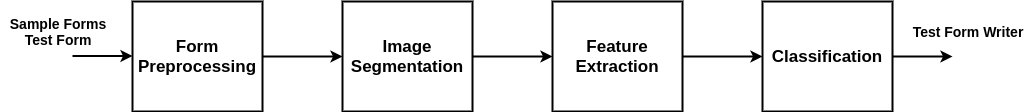
\includegraphics[width=\textwidth]{../figures/pipeline-diagram.png}
    \captionof{figure}{System Pipeline}
    \label{fig:pipeline}
\end{figure*}


